\documentclass{article}
\usepackage{graphicx} % Required for inserting images
\usepackage{float}
\usepackage[T1]{fontenc}
\usepackage{amsmath}
\usepackage[margin=1in]{geometry}
\usepackage{booktabs}
\usepackage{tabularx}
\usepackage[hidelinks]{hyperref}

\title{Holding shorts to the time exit on the short-only book}
\author{Experiment report \textperiodcentered{} L/S Gamma Desk, QUANTT}
\date{2026-10-16}

\begin{document}

\maketitle

\textbf{Question:} On the short-only book, does removing the flat-signal exit raise net P\&L at 1x and 2x spreads, in both halves, without a worse daily tail?

\textbf{Method:}

\begin{itemize}

\item \textbf{Pre-registration:} the hypothesis card was committed before any run (commit dbf1d11).

\item \textbf{Data:} the live paper rules (\texttt{configs/\allowbreak{}paper.\allowbreak{}toml}) are replayed on R2 replay snapshots v1 (config\_hash b040760187f0) over the development window 2014-06-02 to 2024-12-31. The hold-out (2025-01-01 to 2026-07-10) was not used.

\item \textbf{Book:} short-only (\texttt{[signal] long\_\allowbreak{}band = -\allowbreak{}inf}): a short put near 30 DTE, 1 contract, hedged daily at 10:15 ET. A long signal never fires on this book, so there is no flip exit.

\item \textbf{Variants:}

\begin{itemize}

\item \texttt{short\_\allowbreak{}only} (reference): the 3-day flat exit. Same config as \texttt{2026-\allowbreak{}10-\allowbreak{}16-\allowbreak{}short-\allowbreak{}only/\allowbreak{}short\_\allowbreak{}only}.

\item \texttt{no\_\allowbreak{}flat} (primary): \texttt{flat\_\allowbreak{}days = 999}, so shorts close only at 7 DTE, on the stop (1x credit) or at the 50\% profit-take.

\item \texttt{flat10} (sensitivity, reported only): \texttt{flat\_\allowbreak{}days = 10}.

\end{itemize}

\item \textbf{Runs:} every variant ran once at 1x and 2x spreads. Costs are \$0.65 per contract and \$0.005 per share, with a \$1 minimum per order.

\end{itemize}

This report was written by Claude at the PM's request.

\section{Result vs the pass bar}

\texttt{no\_\allowbreak{}flat} against \texttt{short\_\allowbreak{}only} at the same spread multiple. P\&L is net USD on daily equity for 1 contract. ES is the mean of the worst 5\% of daily P\&L.

\begin{center}\small
\begin{tabularx}{\linewidth}{>{\raggedright\arraybackslash}X l l l l >{\raggedright\arraybackslash}X}
\toprule
\textbf{Check} & \textbf{1x value} & \textbf{1x bar} & \textbf{2x value} & \textbf{2x bar} & \textbf{Result} \\
\midrule
Net P\&L, full window & \ensuremath{-}676 & > \ensuremath{-}774 & \ensuremath{-}2,388 & > \ensuremath{-}2,351 & pass 1x, fail 2x \\
Net P\&L, 2014-06 to 2019-12 & \ensuremath{-}1,023 & > \ensuremath{-}875 & \ensuremath{-}1,540 & > \ensuremath{-}1,261 & fail \\
Net P\&L, 2020-01 to 2024-12 & +347 & > +101 & \ensuremath{-}849 & > \ensuremath{-}1,090 & pass \\
abs ES 5\% \ensuremath{\leq} 1.10 \ensuremath{\times} reference & 91.2 & \ensuremath{\leq} 94.1 & 99.8 & \ensuremath{\leq} 101.7 & pass \\
Event floor: time exits (1x) & 76 & \ensuremath{\geq} 20 &  &  & met \\
\bottomrule
\end{tabularx}
\end{center}

\textbf{Verdict: failed.} Holding shorts to the time exit helps a little at 1x (+\$98 over the full window) but loses at 2x (\ensuremath{-}\$37). It is worse in 2014-2019 at both spreads. The book still loses money in every variant.

\subsection{Full-window numbers (not part of the bar)}

\begin{center}\small
\begin{tabularx}{\linewidth}{>{\raggedright\arraybackslash}X >{\raggedright\arraybackslash}X l l >{\raggedright\arraybackslash}X l l}
\toprule
\textbf{} & \textbf{short\_only 1x} & \textbf{no\_flat 1x} & \textbf{flat10 1x} & \textbf{short\_only 2x} & \textbf{no\_flat 2x} & \textbf{flat10 2x} \\
\midrule
Net P\&L & \ensuremath{-}774 & \ensuremath{-}676 & \ensuremath{-}931 & \ensuremath{-}2,351 & \ensuremath{-}2,388 & \ensuremath{-}2,514 \\
Round-trip P\&L before commissions & +318 & +1,166 & +766 & \ensuremath{-}1,240 & \ensuremath{-}536 & \ensuremath{-}805 \\
Sharpe on \$250k & \ensuremath{-}0.15 & \ensuremath{-}0.13 & \ensuremath{-}0.18 & \ensuremath{-}0.42 & \ensuremath{-}0.45 & \ensuremath{-}0.47 \\
Max drawdown & 2,220 & 1,816 & 2,009 & 3,222 & 3,355 & 3,534 \\
ES 5\% (daily) & \ensuremath{-}85.5 & \ensuremath{-}91.2 & \ensuremath{-}91.7 & \ensuremath{-}92.4 & \ensuremath{-}99.8 & \ensuremath{-}99.3 \\
Round trips & 100 & 76 & 78 & 100 & 76 & 78 \\
Average hold (days) & 10.7 & 23.6 & 20.8 &  &  &  \\
Hedge orders (= hedge fees, USD) & 770 & 1,188 & 1,097 & 770 & 1,188 & 1,097 \\
\bottomrule
\end{tabularx}
\end{center}

\section{Charts}

\begin{figure}[H]\centering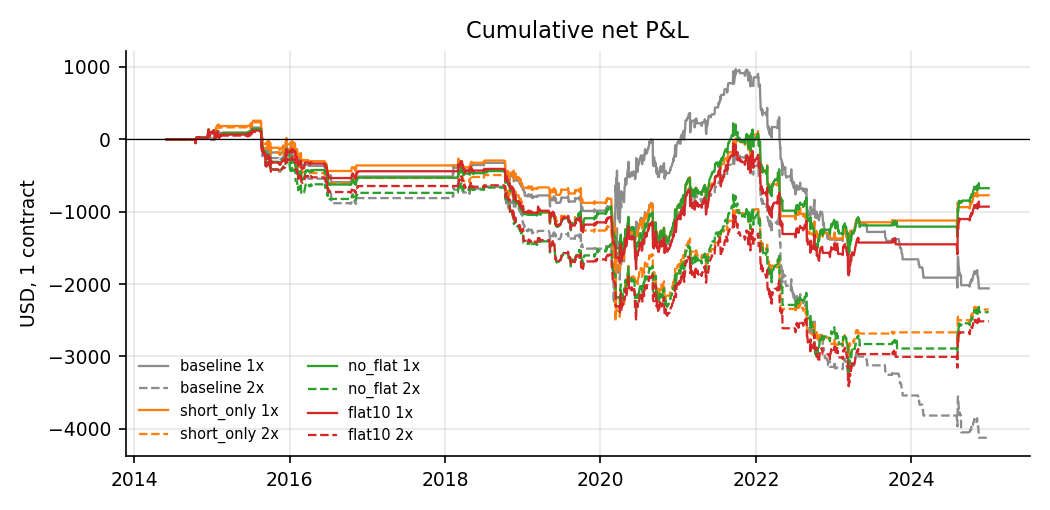
\includegraphics[width=0.92\linewidth]{figures/cum_pnl.png}\caption{Cumulative net P\&L, 1x solid and 2x dashed; baseline (live rules) grey}\end{figure}

\texttt{no\_\allowbreak{}flat} falls behind \texttt{short\_\allowbreak{}only} in 2015-2016 and again in 2018, then catches up in 2019-2024. Most of the catch-up comes in 2022, where it loses \$268 less at 1x. At 2x the lines end almost together.

\begin{figure}[H]\centering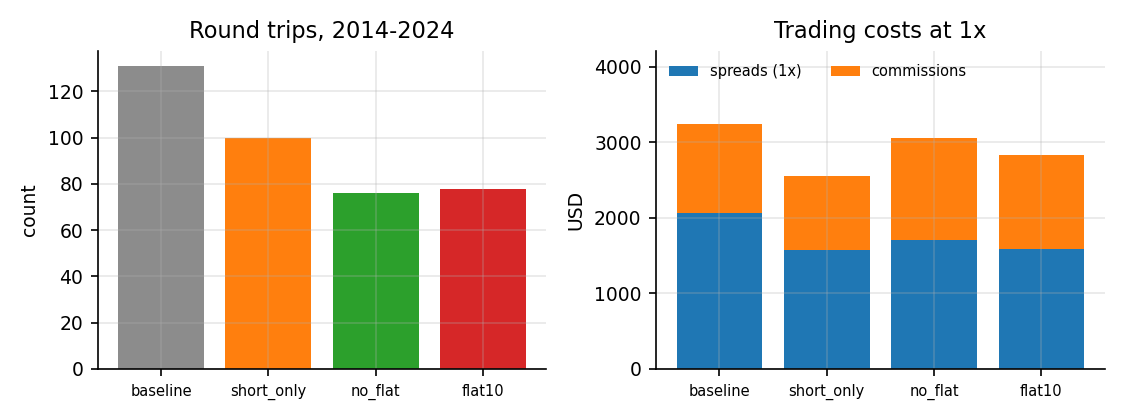
\includegraphics[width=0.92\linewidth]{figures/turnover.png}\caption{Round trips and trading costs at 1x}\end{figure}

This chart shows the cost side. Round trips fall from 100 to 76, but total trading costs rise from about \$2,550 to \$3,050 at 1x: commissions are up \$370 (hedges +\$418, options \ensuremath{-}\$48) and spreads are up \$134.

\begin{figure}[H]\centering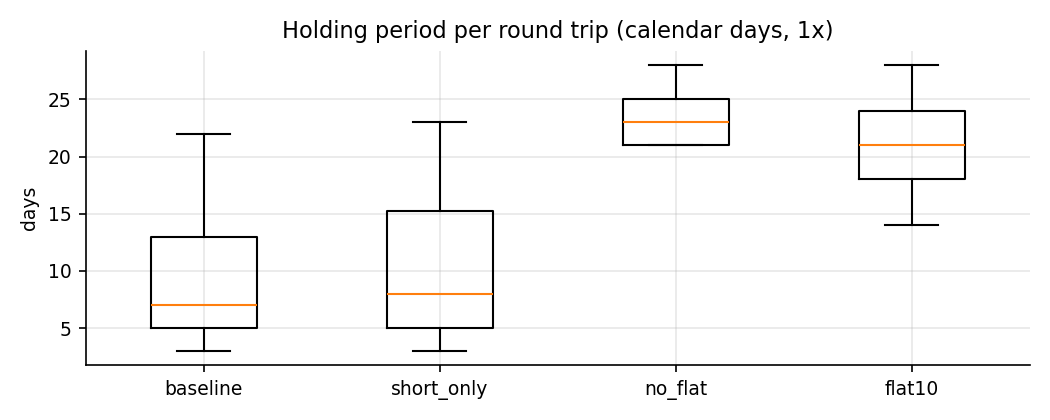
\includegraphics[width=0.92\linewidth]{figures/holding.png}\caption{Holding period per round trip}\end{figure}

Without the flat exit every short is held from entry near 30 DTE to the 7-DTE exit: median 23 days, 5th-95th percentile 21-28. \texttt{flat10} sits in between. The reference's median hold is 8 days.

\begin{figure}[H]\centering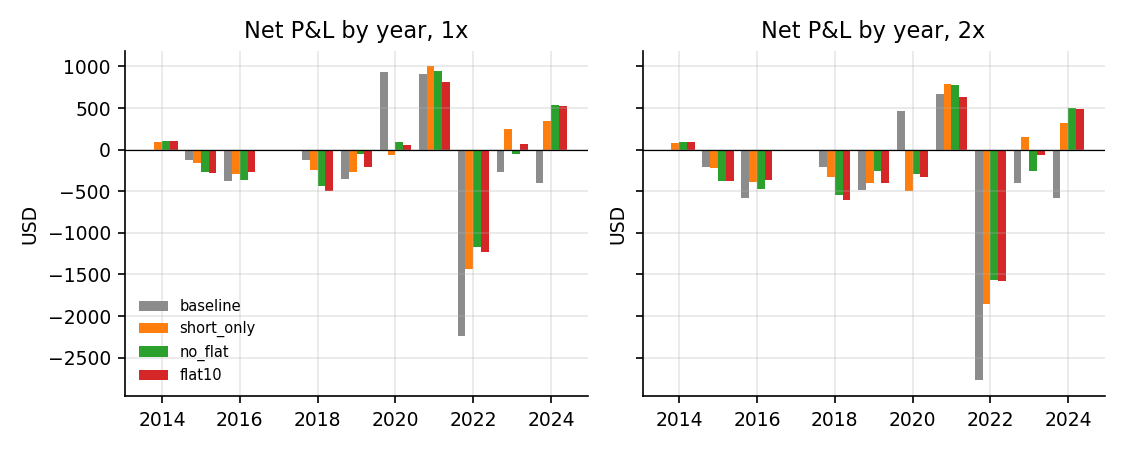
\includegraphics[width=0.92\linewidth]{figures/yearly.png}\caption{Net P\&L by year}\end{figure}

At 1x, holding longer helps in 2014, 2019 (\ensuremath{-}\$56 vs \ensuremath{-}\$270), 2020 (+\$90 vs \ensuremath{-}\$60), 2022 (\ensuremath{-}\$1,165 vs \ensuremath{-}\$1,433) and 2024 (+\$531 vs +\$349). It hurts in 2015-2016, 2018 (\ensuremath{-}\$437 vs \ensuremath{-}\$244), 2021 (+\$948 vs +\$1,000) and 2023 (\ensuremath{-}\$57 vs +\$244). The first-half shortfall comes from 2015-2016 and 2018 (\ensuremath{-}\$381 together), partly offset by 2019 (+\$214).

\begin{figure}[H]\centering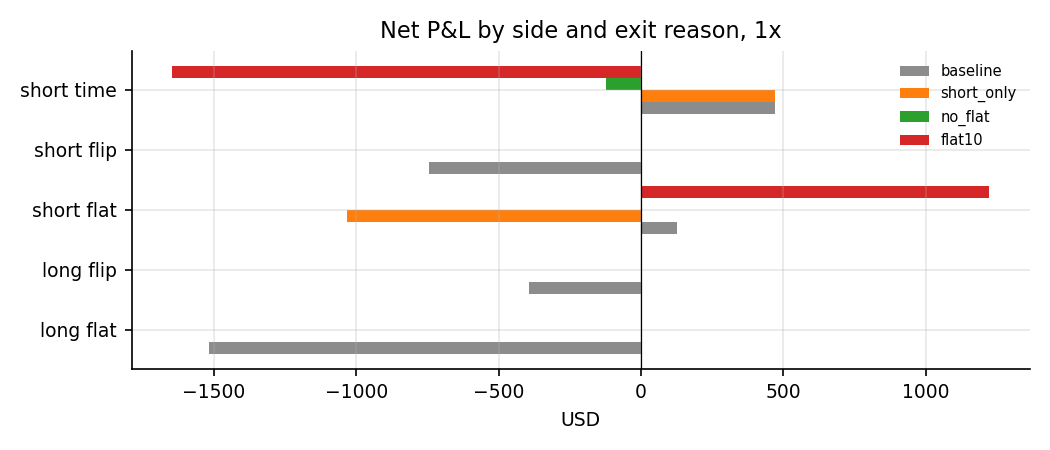
\includegraphics[width=0.92\linewidth]{figures/by_reason.png}\caption{Net P\&L by side and exit reason, 1x}\end{figure}

Every \texttt{no\_\allowbreak{}flat} trade closes at the time exit (no stop or profit-take fired): 76 trades, \ensuremath{-}\$124 net in round trips. The reference's +\$470 from 13 time exits did not scale. Holding every short to 7 DTE also holds the ones that are going wrong.

\begin{figure}[H]\centering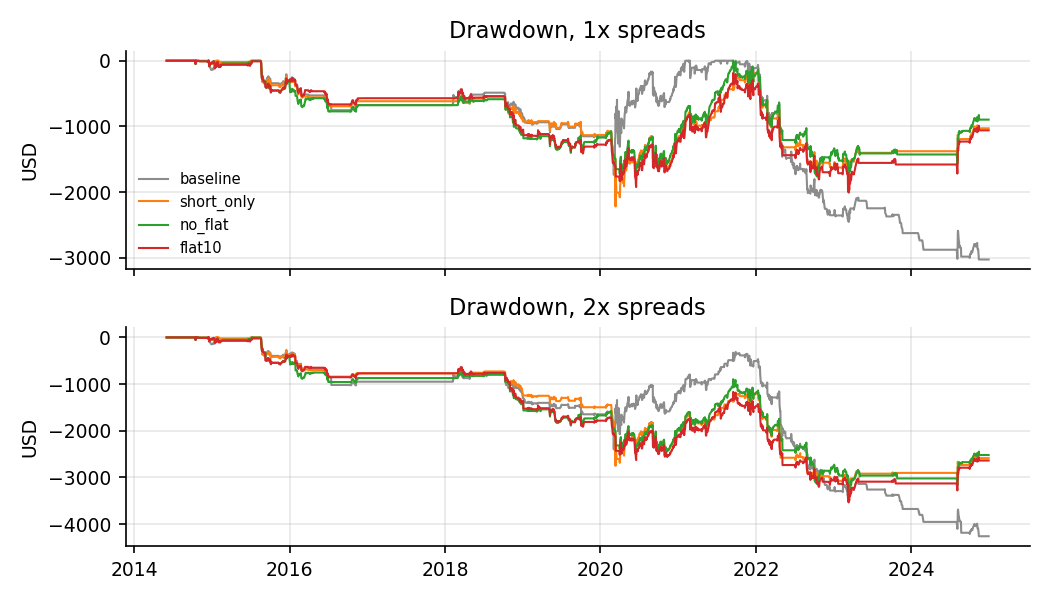
\includegraphics[width=0.92\linewidth]{figures/drawdown.png}\caption{Drawdown at 1x and 2x spreads}\end{figure}

The 1x maximum drawdown is smaller (\$1,816 against \$2,220). That is because the 2015-2020 decline was shallower, helped by 2019-2020. The reference's maximum drawdown runs from mid-2015 to the March 2020 trough. \texttt{no\_\allowbreak{}flat}'s comes later (2021-09 to 2023-03), and over that stretch it is actually deeper than the reference's (\$1,816 against \$1,724). At 2x it is slightly larger overall.

\begin{figure}[H]\centering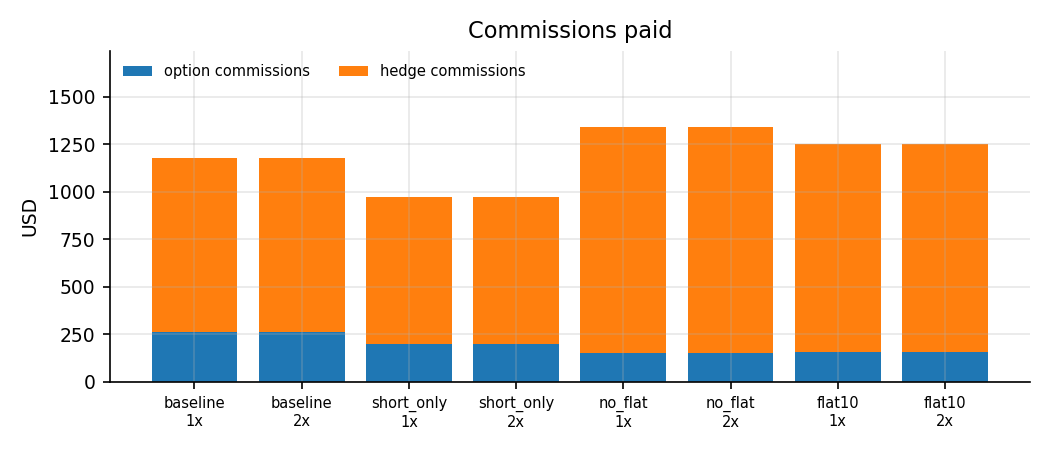
\includegraphics[width=0.92\linewidth]{figures/fees.png}\caption{Commissions paid}\end{figure}

Hedge commissions are most of the commissions in every short-only variant. Spreads (the turnover chart) are the larger cost overall.

\section{Analysis}

The hypothesis had two parts. Shorts would keep more of the late time decay, and they would pay fewer spreads. The first part held: round-trip P\&L before commissions rose from +\$318 to +\$1,166 at 1x (3.7x). That figure is already net of the spreads paid inside each round trip. The second part did not hold. The 1x bridge from the reference to \texttt{no\_\allowbreak{}flat} is: +\$848 more round-trip P\&L, \ensuremath{-}\$410 more commissions attributed to round trips, \ensuremath{-}\$340 more unattributed unwind cost, giving +\$98. At 2x it is +\$704 \ensuremath{-} \$410 \ensuremath{-} \$330 = \ensuremath{-}\$37.

\begin{itemize}

\item \textbf{More hedge orders.} A short held for 24 days instead of 11 is hedged on more days. With 1 contract, each small daily hedge pays the \$1 order minimum. Hedge orders rose from 770 to 1,188 (+\$418), while shares traded fell about 6\% (12,204 against 13,046 for the reference). So the extra cost is the fixed order minimum, not hedging volume. The 10-share hedge band from \texttt{2026-\allowbreak{}10-\allowbreak{}16-\allowbreak{}hedge-\allowbreak{}band} targets exactly this cost.

\item \textbf{Costlier closes, already inside the round-trip P\&L.} The option-leg spread cost rose from \$1,512 to \$1,651 (+\$139) despite 24 fewer round trips. Holding to 7 DTE ends more shorts in the money (32\% against 27\%), and an in-the-money round trip costs far more to cross: about \$56 against \$38 for the reference's in-the-money round trips, and about \$6-7 out of the money. The spread model fits a wider cost for deep-in-the-money options, and the 2x run doubles it. This cost is part of why the gross gain is \$848 and not more.

\item \textbf{Unwind cost, and most of it is noise.} About \$552 at 1x is not attributed to any round trip, against \$212 for the reference. It is the order that flattens the hedge after each close: a \$1 commission plus the gap between the fill-window spot and the decision spot, times the shares. \texttt{no\_\allowbreak{}flat} had fewer such orders, not bigger ones: 50 averaging 39 shares, against 90 averaging 44, because 25 of its closes re-entered at once and carried the shares over. The growth comes from the price gap: \$502 against \$122. A few days in 2020 and 2022 dominate (the five worst unwinds total more than the whole \$502, and the median is about \$0). The pass bar uses equity P\&L, which includes it.

\end{itemize}

So the decay gain is real, and the flat exit was costing the book something. But on a 1-contract book with daily hedges, the extra \$1 hedge orders take about half of the gain, and the unwind noise takes most of the rest. The 2x shortfall (\$37) and the 1x gain (\$98) are both smaller than the noise in a handful of unwind fills. The honest reading: on this cost structure, holding to the time exit is roughly neutral, not a clear improvement.

\section{Verdict}

\textbf{Failed} on the pre-registered bar: the 2x full window and the 2014-2019 half fail. Keep the live 3-day flat exit for now.

A follow-up worth pre-registering, which needs its own card and is in-sample: \texttt{no\_\allowbreak{}flat} combined with the 10-share hedge band, which cuts the cost that grew here. Its reference should be short-only plus the 10-share hedge band (queued as ``short-only + hedge band'').

\section{Caveats}

\begin{itemize}

\item \textbf{In-sample:} the idea came from the baseline's exit-reason breakdown on this same window.

\item \textbf{One contract:} the \$1 order minimum turns longer holds into many small hedge orders. With more contracts per position the hedge orders would be larger and that cost would matter less.

\item \textbf{Spread model:} fitted on about two weeks of calm 2026 live quotes. The in-the-money spread tier drives part of this result, and the 2x run is the stress test.

\item \textbf{Data gaps:} R2 has no month-end weekdays, so 89 scheduled times (3.3\%) are skipped in every variant.

\item \textbf{Few events per year:} 31 trades in 2014-2019 and 45 in 2020-2024 for \texttt{no\_\allowbreak{}flat}. The yearly differences rest on a handful of trades each.

\item \textbf{Unwind noise:} the hedge-flattening orders fill on a spot price 15-30 minutes after the decision spot, and a few such fills are larger than the margins in this test.

\end{itemize}

\section{Trials}

6 trials for this experiment (3 variants at 1x and 2x, one run of \texttt{experiment.\allowbreak{}py}), plus the baseline's 2. \texttt{short\_\allowbreak{}only} repeats the config of \texttt{2026-\allowbreak{}10-\allowbreak{}16-\allowbreak{}short-\allowbreak{}only/\allowbreak{}short\_\allowbreak{}only} (2 earlier trials). Its numbers here are identical: \ensuremath{-}\$773.8 at 1x, \ensuremath{-}\$2,351.3 at 2x. So across the desk the same short-only test is registered 4 times. The pass bar was not changed.

\end{document}
